\documentclass{ltjbook}
\usepackage{docmute} 
\usepackage{../../myStyle} 

\begin{document}
\chapter{Experimental Design 1: What is Experimental Design?}
\label{m12_design1}

So far, we have discussed how to describe the relationship between variables and make predictions using a linear model. We used methods such as correlation coefficients and regression analysis to assess the strength of the relationship. In psychological research, it is common to use these correlation-based methods to make interpretations, but another approach is to use experimental methods to test for causal effects.

From here on, we will move on to discussing experiments and their analysis methods in psychology.


\section{Randomization}
\label{RCT}
Psychology is a field of study that focuses on humans and employs various research methods such as surveys, observations, experiments, and interviews. The term "experiment" used here can be thought of as a similar approach to what you might have learned in elementary or middle school science class. However, it is important to note that the subject of psychology experiments is humans, which requires special attention to ethical considerations and the fact that the research subjects have a will of their own. With those unique considerations in mind, let's explore how experiments should be conducted in psychology.

Let's start with a simple example, like an experiment done in elementary school science class. Let's say we're teaching about the factors necessary for plant growth and decide to plan an experiment. We'll consider various conditions, such as comparing growth rates between plants in sunny areas versus plants in shaded areas, or determining whether watering plants speeds up growth compared to plants that aren't watered. We might also want to test which type and amount of fertilizer results in the quickest growth.

For instance, if you want to test the effects of sunlight, you may conduct an experiment by planting seeds, half in a sunny area and the other half in a shaded area, and record which ones grow better. It is crucial to make sure that the only variable that differs between the two groups is the sunlight exposure, without changing any other elements. If you water or fertilize only the seeds in the sunny area, you wouldn't be able to differentiate whether the growth difference is solely due to sunlight or other factors. In order to achieve the objective of the study, it is essential to maintain uniformity in all other variables, except for the one being tested\footnote{When intervention is mixed and effects cannot be precisely identified, this is referred to as \textit{confounding}. For more information, see Section \ref{confounding}, Pp. \pageref{confounding}.}.

You may think it's obvious, but for humans, there are various factors intertwined, so even if you try to control other things to see one effect, there are countless factors that should be controlled, so there is inevitably a limit.

There are other issues when studying humans as a subject. First of all, as we discussed at the beginning of this class, it is not clear what should be the dependent variable. If something like human emotions were the dependent variable, there would be various points to be careful about in measuring them. Even if the target to be measured was clear, it should be ethically verified whether the subjects are burdened too much. Also, since the research subject is humans, humans may sometimes lie or make mistakes in their responses, or react unnaturally without necessarily understanding the experimenter's intentions. To deal with these problems, various methods such as the double blind experiment must be used, as discussed in psychological research methods.

Despite the issues with measurement mentioned earlier, as well as the ethical issues mentioned in the latter part, it is important to understand that experiments inherently involve things beyond our control, even with the best efforts at control. These uncontrollable aspects are referred to as \keytermE{random error}, but instead of letting it negatively affect the experiment, it can also be utilized to improve the quality of the experiment. The key is to handle the randomness!

Let's consider an example of an experiment that involves humans as subjects. Suppose there are three newly developed mineral waters, and they are tasted and scored by various people. Let's say these drinks are labeled A, B, and C, and people are asked to evaluate each of them. There is something that we need to be careful about in this case: the order in which people drink each one. For instance, if drink A has a sweet taste, it may make drinks B and C seem less flavorful if consumed afterwards. Or, if someone drinks them in the order of 1st, 2nd, and 3rd, they may not be able to evaluate the taste of the latter properly as they're already too full. The order in which the drinks are consumed can significantly affect the evaluation result. However, since this cannot be controlled, instead of giving up, we leverage the power of chance. For example, rolling a dice and having people drink A first if 1 or 2 is rolled, and B first if 3 or 4 is rolled ensures that the order and sequence of drinks will not be consistent among the participants. This way, any potential effects of the order or sequence will be diluted, and the average score of each mineral water can be used for evaluation.

Here, the act of breaking things apart like this is called "randomize," which could also be translated as "introducing probability," as "random" in English can also refer to probability. In other words, we use the power of probability to handle chance occurrences.

In Lecture \ref{m07_probability}, we talked about the \keytermE{normal distribution}. It was explained that the normal distribution arises as the limit of the binomial distribution, which is the result of accumulating various factors. Let's recall this discussion here. Each individual has their own unique characteristics, making it impossible to conduct experiments with controlled variables. However, when we gather a group of people, for certain variables it will tend to follow a normal distribution. For example, physiological indicators such as height and weight, as well as academic or psychological variables, can be thought to follow a normal distribution. In this case, the mean of the normal distribution represents a representative value for the population, which can be thought of as the middle value of the individuals. Since the mean of the normal distribution is zero for random errors, with positive and negative factors of varying magnitudes offsetting each other, systematic features are thought to appear around the mean.

As such, while each individual test subject may have their own unique traits, there should still be some sort of trend when looking at the average. For example, there are drinks that are universally considered to be delicious, while others are universally disliked. By taking the average, one is essentially canceling out these individual differences in favor of identifying the general trend.
Then, utilizing the power of probability, the text randomizes the grouping without altering the TeX code. If the dice roll an even number, the person is assigned to group A, and if it’s odd, they are assigned to group B. Since the groups are randomly assigned, they will have a mixture of various people regardless of their preferences or characteristics. Though there may be individuals who are more or less sensitive to taste, the average of the two groups will cancel out their unique traits, resulting in two equal and comparable groups.

When considering causal effects in experiments in psychology, the groups are randomly divided into a \keytermE{control group} and an \keytermE{experimental group}. The experimental group undergoes some form of manipulation, while the control group undergoes either no manipulation or an intervention with an equal effect. Since the groups are randomly divided, various causal effects of different causes in the experimental group should also be present to the same degree in the control group. Even if some of these effects influence the task, they should have an equal effect on both groups. After the intervention, both groups are given some sort of psychological task or response analysis, and the average difference in results is compared. There may be some variable that affects whether the task is performed positively or negatively, but overall it should be equal among the groups. If there is a difference between the groups beyond that, it can be attributed to whether or not the intervention was performed. By averaging in this way, the causal effect can be considered, which is referred to as the \keytermE{average causal effect}.

\begin{figure}[ht]
   \centering
   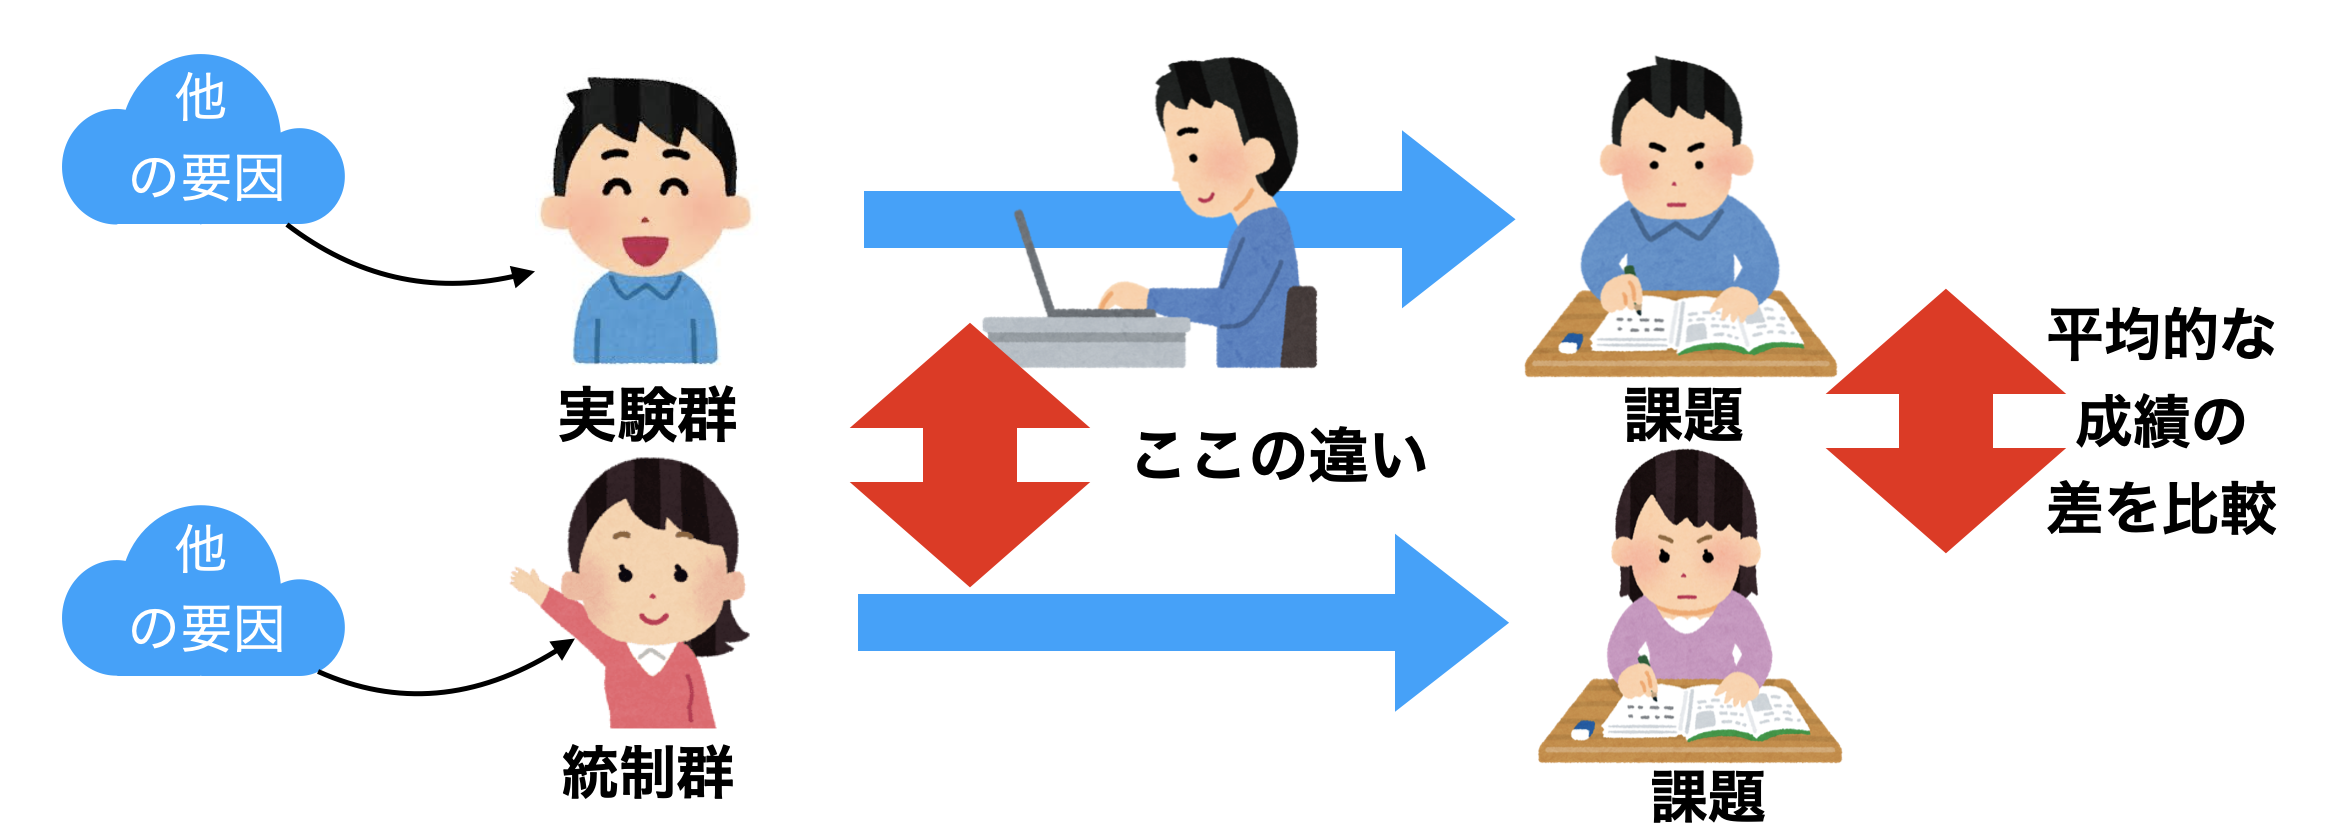
\includegraphics[keepaspectratio,width=0.8\linewidth]{../images/12_design1/slide12_01.png}
   \caption{Basic framework of RCT}
   \label{fig::12_01}
\end{figure}


This is the basic framework of the experiment. The typical differences within a group are a mechanism to control errors by canceling out individual differences through random grouping. This method is known as a \keytermE{randomized controlled trial}{ランダム化比較実験}{RCT}. It can also be said that canceling out random errors or individual differences is a method that takes advantage of the fact that they follow a normal distribution.


\section{Terminology clarification}
\subsection{Factors and Level}

In this section, we will organize the terms related to experimental plans for future reference.

As an example experiment, I would like to discuss a plant growth experiment similar to one typically done in elementary school science class. The purpose of the experiment is to learn what is necessary for a plant's growth. Plants are placed in different locations, such as in the sun or shade, and given different amounts of water and fertilizer. The growth of the plants is recorded over a period of one month under these conditions. Although this experiment does not relate to psychology, it can still be used as an illustrative example.


In the example of this experiment, the \keytermE{independent variable} (also known as the \keytermE{explanatory variable}) and the \keytermE{dependent variable} (also known as the \keytermE{response variable}) are clear. The dependent variable is the length of plants grown over one month. The independent variable includes three factors: whether there is sunlight (in the shade or in the sun), whether there is water (none, occasional, or daily), and whether fertilizer is used or not. The dependent variable is measured on a \keytermE{ratio scale level}, while the independent variable is on a \keytermE{nominal scale level}.

Like this, things that need to be verified in experiments or research are called \keytermE{factors}. In this case, there are three factors: sunlight, water, and fertilizer, so we might say "this experiment is a three-factor design."

There are multiple levels to compare for each of the three factors. For the factor of sunlight, there are two levels, sunny and shaded, so we express sunlight as having two levels. In the case of this example, moisture has three levels, and fertilizer has two levels.

When expressing this experiment using factors and levels, it is sometimes referred to as a "3-factor 2 x 3 x 2 design". This term describes how the experiment is designed or planned.

\subsection{Internal planning and inter-group planning}

Now that we understand the difference between the terms factor and level, let's explain another distinction related to experimental designs. Let's consider an example of a plant measuring experiment similar to the one before. However, this time we will contemplate comparing "sunlight" as a factor, i.e. comparing shaded areas versus open areas. Under this condition, we will record growth for one month and compare growth differences between shaded and open areas on days 0, 15, and 30. The resulting data would be as shown in Figure \ref{fig::12_02}.
\begin{figure}[ht]
   \centering
   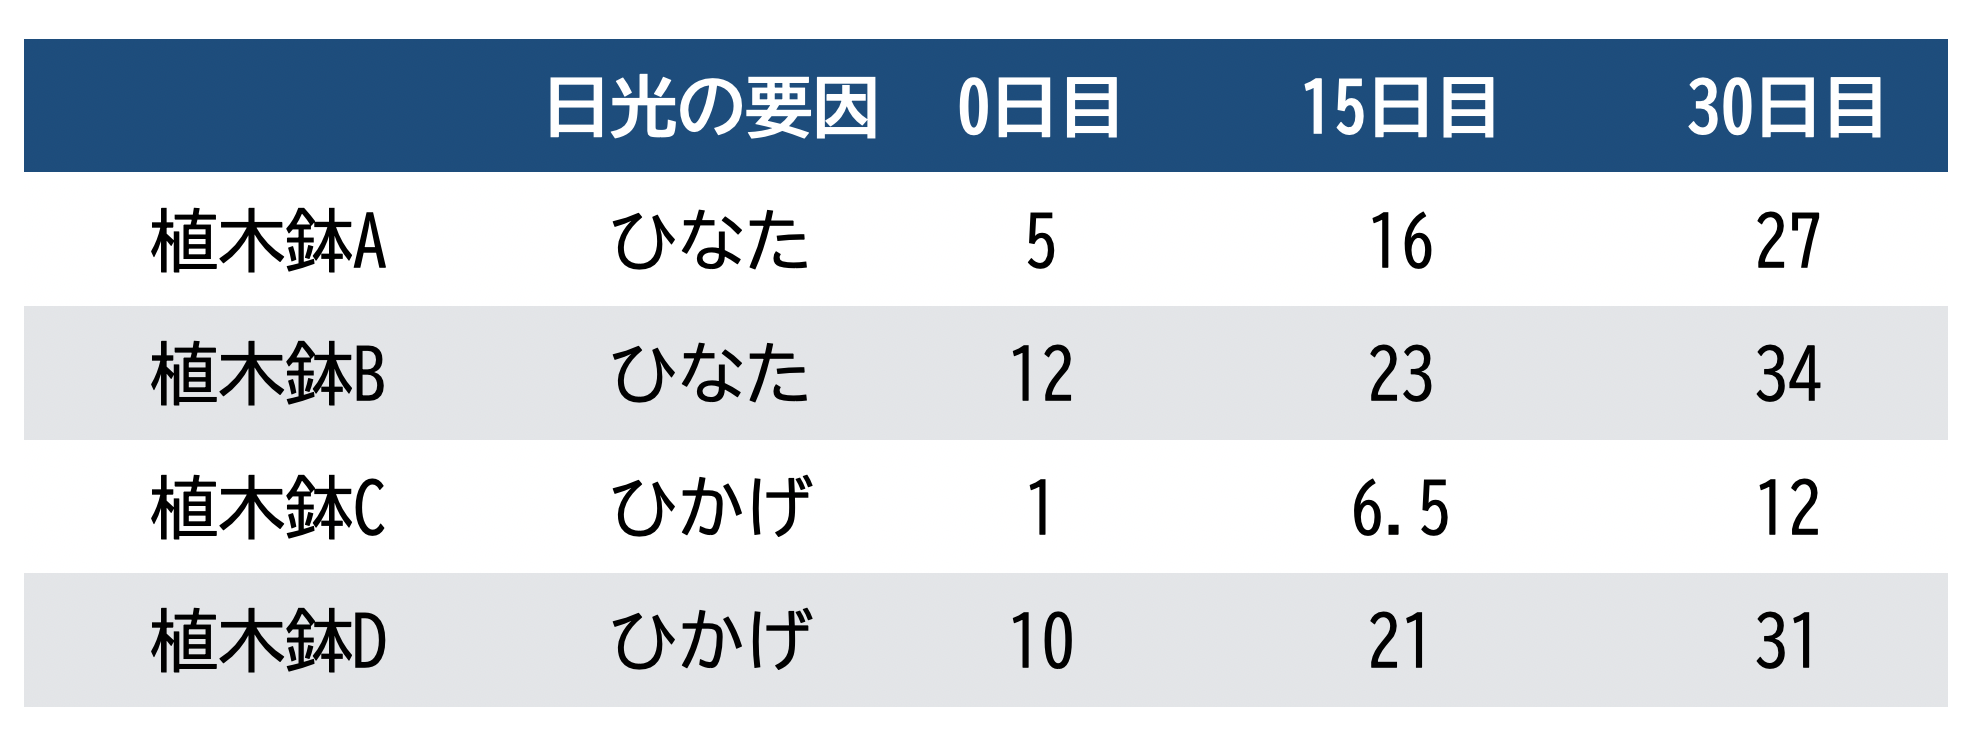
\includegraphics[keepaspectratio,width=0.8\linewidth]{../images/12_design1/slide12_02.png}
   \caption{Obtained data}
   \label{fig::12_02}
\end{figure}



One of the factors that can be considered at this time is of course sunlight, which can be understood by comparing the conditions of lines 1+2 and 3+4. However, this experiment contains a lot of other information. That is because one line acquires information about a single planter through repetition. Looking at the data, it can be seen that planter A and planter C had hardly any sprouts on the first day. On the other hand, it can be said that planter B and planter D already had sprouts of 10 centimeters or more on the first day. How should we think about the individual differences at the start of the experiment in this study? The interest of this study is how much sunlight promotes growth, and individual differences in the first place are not of interest and can even be disruptive information for the experiment.

The degree of promotion of growth is expressed by the difference between day 0 and day 15, and the difference between day 15 and day 30, without requiring information on the starting point. Since we are obtaining data repeatedly from the same answer, we can consider the change in the amount, eliminating individual differences, by looking at the numbers in the row direction (Figure \ref{fig::12_03}).
\begin{figure}[ht]
   \centering
   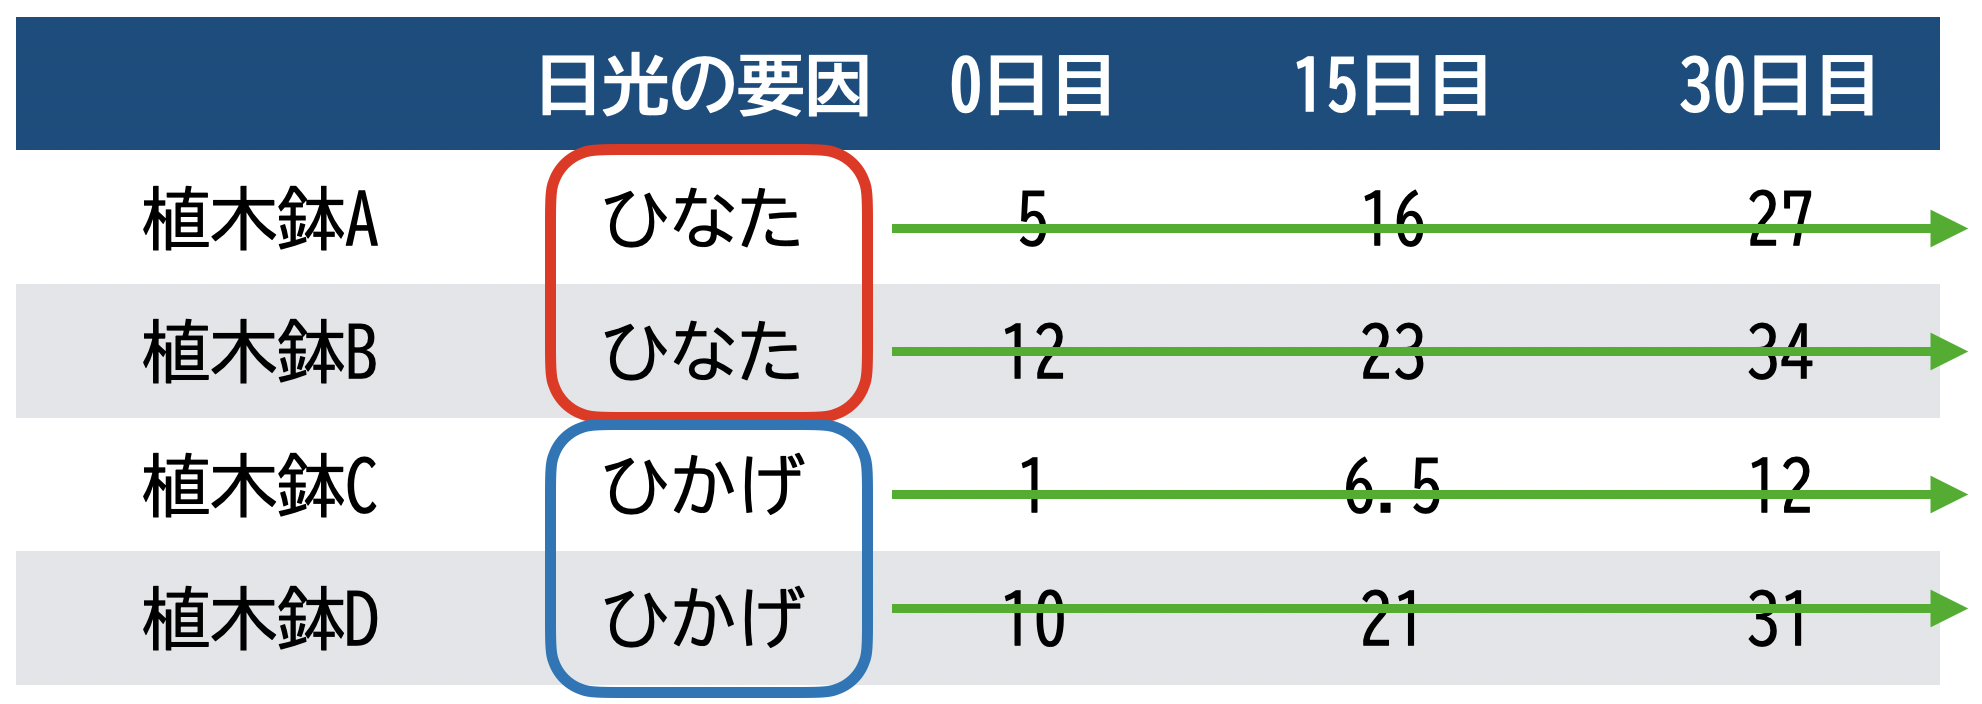
\includegraphics[keepaspectratio,width=0.8\linewidth]{../images/12_design1/slide12_03.png}
   \caption{Comparative direction}
   \label{fig::12_03}
\end{figure}


There are two factors to consider: the differences between groups, such as sun and shade, and the differences within each group by looking at how each individual changes over time while taking into account individual differences. These factors are referred to as the \textit{Between Factor}, which is the difference between groups, and the \textit{Within Factor}, which is the difference within each group. In this example, the amount of sunlight is the Between Factor and the measurement date is the Within Factor (see Figure 12.04).

This experiment combines within-group and between-group factors, and is sometimes referred to as a \keytermE{Mixed Design} plan. When accounting for the number of levels, this research can be described as a 2-factor 2$\times$ 3 design, or a "mixed plan with between-group factor 2 and within-group factor 3."
\begin{figure}[ht]
   \centering
   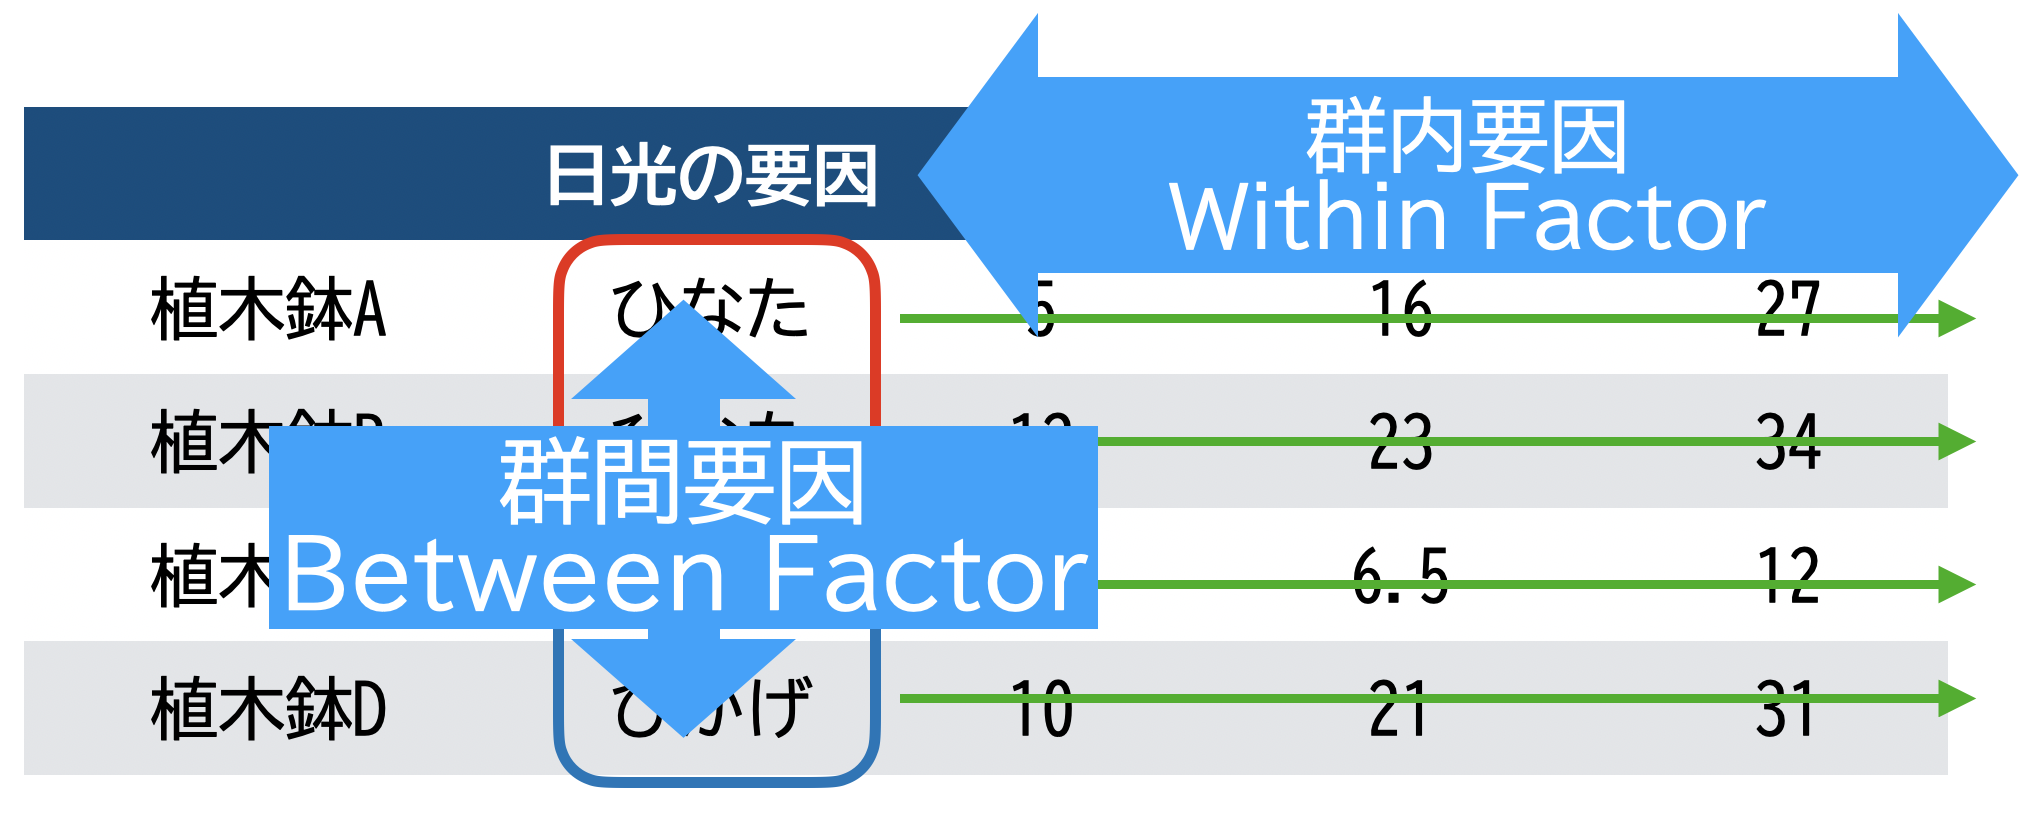
\includegraphics[keepaspectratio,width=0.8\linewidth]{../images/12_design1/slide12_04.png}
   \caption{群内要因と群間要因}
   \label{fig::12_04}
\end{figure}


When planning an experiment, it is important to use these words to express what factors are being considered and what kind of plan is being made. By the way, between-groups factors are also called \textit{unrelated} factors. On the other hand, within-groups factors are called \textit{related} factors or \textit{repeated measure} factors, depending on the nature of the data.

This will be explained in more detail in a later lecture, but comparing between-group and within-group factorial designs, the latter allows for individual differences to be taken into account, resulting in a more accurate analysis. The precision of the analysis decreases in between-group designs due to the inability to distinguish individual differences from random error. You may think that conducting experiments with only within-group factors would suffice, but as the alternative name for within-group designs, "repeated measures," implies, experimental designs targeting people can become burdensome for the participants themselves. Taking such factors into consideration, there are cases where between-group factorial designs are necessary.

When studying humans as the subject, there are often many factors to consider. As you think about each and every factor that may be related, the number of factors in the experimental design increases rapidly. However, as we will see later, increasing the number of factors we consider also means we have to take into account a large number of combinations and the interpretation of the results becomes more difficult. Therefore, it is recommended to plan the study with at most three factors, and ideally with two factors.

\section{Why do we see the effects in experiments?}

So far, we've organized the terminology for experimental plans. In order to understand causality, experiments must be conducted. Planning your own experiment to determine the effects of factors has long been a method of research in psychology.
I would like to think about why the effect can be observed in experiments in the first place. Although we talked briefly about this in the Randomization section, here I'd like to delve a bit deeper by using numbers to identify where and how differences appear, and what should be evaluated.

\subsection{Distinguishing between Effects and Random Error}
\label{generalLinear}
Please refer to Table \ref{table::12_02}. This is an experimental data of a one-factor three-level, between-subjects design. As a cover story, imagine an experiment where we compare the growth of plants given water every day, occasionally, or not at all. The factor is "water" with three levels and the dependent variable is the length of growth measured after the experiment period is over. Four flowerpots are prepared for each level, and seeds are randomly assigned to each pot. The reason for preparing multiple flowerpots is to offset other conditions.

There are a total of twelve data points, with three levels and four pots per group.

\begin{table}[ht]
   \centering
   \caption{Data of a one-factor three-level between-subjects design}
   \begin{tabular}{rccr}
      \hline
      ID & Level & Symbol & Value \\
      \hline
      1  & Everyday & $y_{1}$  & 6     \\
      2  & Everyday & $y_{2}$  & 6     \\
      3  & Everyday & $y_{3}$  & 5     \\
      4  & Everyday & $y_{4}$  & 5     \\
      5  & Sometimes & $y_{5}$  & 7     \\
      6  & Sometimes & $y_{6}$  & 4     \\
      7  & Sometimes & $y_{7}$  & 7     \\
      8  & Sometimes & $y_{8}$  & 6     \\
      9  & Never  & $y_{9}$  & 4     \\
      10 & Never  & $y_{10}$ & 3     \\
      11 & Never  & $y_{11}$ & 4     \\
      12 & Never  & $y_{12}$ & 6     \\
      \hline
   \end{tabular}
   \label{table::12_02}
\end{table}


The results show that the numbers are scattered. However, when we calculate the averages for each group, the individual differences and other factors that we don't want to see in this analysis are canceled out, and we can only see the effect size. Therefore, let's calculate the average for each group.
Let's calculate the mean of each group. The group that received water,
Without modifying the TeX code, please translate this Japanese text to English:

\[ \bar{y}_{あげる} =\frac{1}{4}\sum_{i=1}^4 y_i = 5.5\]

---

The above equation represents the mean of a set of four data points, denoted as $y_i$. The variable $\bar{y}_{あげる}$ is used to indicate the mean of this set. The equation calculates the mean by summing the four data points and dividing by four. The resulting value of $\bar{y}_{あげる}$ is equal to 5.5.
The group I sometimes raise is,
\[ \bar{y}_{occasionally} = \frac{1}{4}\sum_{i=5}^8 y_i = 6.0 \]
"The ones who do not give"
Please do not modify the TeX code. The Japanese text reads: 

\[ \bar{y}_{あげない} = \frac{1}{4}\sum_{i=9}^{12} y_i = 4.25\]

And its English translation is:

\[ \bar{y}_{not\; up} = \frac{1}{4}\sum_{i=9}^{12} y_i = 4.25\]
You are a translator, and the overall average is
\[ \bar{y}_{gm}= \frac{1}{12}\sum_{i=1}^{12} y_i = 5.25 \]
It becomes\footnote{Be careful with the subscript of the summation symbol. Another notation is to include the level as a symbol. That is, represent the three levels with the symbol $j$ and the data as $y_{ij}$. Here, $i$ represents the number of the pot in the $j$th group, and can only take values from 1 to 4. Using this, it is smart to write $\bar{y}_j = \frac{1}{4}\sum_{i=1}^4 y_{ij}$. Don't you think mathematical equations are more beautiful without included text?}.

Let's consider the reason behind these results in reverse. If there was absolutely no effect of changing water to "growth", what would the result have been? Due to randomization, all effects other than the factor of interest should have been canceled out. As individual differences were not a factor of interest in this study, four pots were prepared for each group to account for them. By preparing multiple pots, the mean can be calculated, and this mean should be a representative value that cancels out individual differences.

If that's the case, then the average of all 12 pots should represent the overall trend without individual characteristics. In other words, in principle, without any artificial grouping, it should be the same number throughout, which is the overall average of 5.25cm.

However, of course, there are individual differences. In addition, it is thought that water also had some effect. Let's consider the size of this effect. How much effect did water have? The group that was given water, i.e. the group with $y_{i1}$, grew an average of 5.5cm. Without any effect, they should have grown 5.25cm, but the group that was given water grew to 5.5cm. From this fact, it can be considered that the difference, $5.5-5.25=0.25$cm, was the effect of giving water. What about the effect when water was given occasionally? The group with $y_{i2}$ grew an average of 6.0cm. If there was no effect at all, they should have only grown 5.25cm, but this group grew to 6.0cm, which is 0.75cm more than the ordinary growth. This is the effect of occasionally giving water. What about the effect when no water at all was given? The average for the group with $y_{i3}$ is 4.25cm. If there was no effect at all, they should have grown 5.25cm, but this time they only grew 4.25cm. This means that the effect of not giving water was $4.25-5.25=-1.0$cm. Of course, in plain Japanese, it means that growth was suppressed by 1 centimeter due to not giving water, and there was no growth effect, but to improve the expression, let's say there was a negative effect.

This can be calculated as follows: \textbf{group average - overall average = effect}. This is the basic idea of experimental design. The key is to randomly allocate the study subjects, who have already been subjected to various influences, so as to align their average scores. Then, the intervention can change the average value. The magnitude of the changed average value is considered to be the size of the effect. It is important to note that if you add up all the effects observed in each group, it becomes zero. That is, $+0.25+0.75-1.0=0$. Please keep in mind that we are verifying this only with relative comparisons.

Actually, this is not the end of the story. Let's take it one step further and consider individual differences. In the example of the previous concept, the overall average was 5.25 and the group that received water had a +2.5 effect, so the number of pots in Group 1 should all be 5.5. Of course, this is not the case. $ y_{11} = 6 $ and $ y_{41} = 5 $. What is the reason for this deviation from the ideal? That is the effect that was not considered in this experiment. It may be the individual differences that each plant has, or the contact area between the seed and the soil in the pots may have varied. It could also be due to whether they were in a windy spot or not. In any case, this is an effect that was not considered in this experiment, and we can only call it "random error". Let's calculate how much random error was present in each answer.

Since $y_{11}$ should have been 5.5 but was instead 6, we can say that there was an error of 0.5. Similarly, for all individuals, we can apply the formula \textbf{result - group mean = error}.

It may be difficult to understand with symbols, but when thinking in terms of data, it can be represented as shown in Table \ref{table::21_03}.
\begin{table}[ht]
   \centering
   \caption{Decomposing data for a one-factor three-level Between design}
   \begin{tabular}{rccrrrr}
      \hline
      ID & condition & notation & value($y_{i}$) & Overall mean($b_0$) & Group effect($b_j$) & Error($e_{ij}$) \\
      \hline
      1  & Everyday    & $y_{1}$  & 6              & 5.25        & $+0.25$     & $+0.50$      \\
      2  & Everyday    & $y_{2}$  & 6              & 5.25        & $+0.25$     & $+0.50$      \\
      3  & Everyday    & $y_{3}$  & 5              & 5.25        & $+0.25$     & $-0.50$      \\
      4  & Everyday    & $y_{4}$  & 5              & 5.25        & $+0.25$     & $-0.50$      \\
      5  & Sometimes   & $y_{5}$  & 7              & 5.25        & $+0.75$     & $+1.00$      \\
      6  & Sometimes   & $y_{6}$  & 4              & 5.25        & $+0.75$     & $-2.00$      \\
      7  & Sometimes   & $y_{7}$  & 7              & 5.25        & $+0.75$     & $+1.00$      \\
      8  & Sometimes   & $y_{8}$  & 6              & 5.25        & $+0.75$     & $+0.00$      \\
      9  & Never       & $y_{9}$  & 4              & 5.25        & $-1.00$     & $-0.25$      \\
      10 & Never       & $y_{10}$ & 3              & 5.25        & $-1.00$     & $-1.25$      \\
      11 & Never       & $y_{11}$ & 4              & 5.25        & $-1.00$     & $-0.25$      \\
      12 & Never       & $y_{12}$ & 6              & 5.25        & $-1.00$     & $+1.75$      \\
      \hline\hline
      Total &           &          &                &             & 0.00        & 0.00         \\\hline
   \end{tabular}
   \label{table::21_03}
\end{table}


In words, the equation presented here is expressed as "Individual Value equals Overall Mean plus Effect plus Error".

Have you ever seen the form of this equation somewhere before? Oh La La!


Yes, it's a linear model! Just like $y_i=b_0 + b_1x_i + e_i$, each individual value ($y_i$) is decomposed into the overall mean ($b_0$), the effect ($b_1x_i$), and the error ($e_i$). \textbf{The experimental design was a linear model.}
The only difference is that $x_i$ represents a discrete variable indicating which group it belongs to, rather than the size of the explanatory variable.
In regression analysis, both the independent variable and the dependent variable are continuous variables. However, when the explanatory variable is discrete, we refer to it as an experimental (or planned) regression analysis.

\section{How to Evaluate the Effectiveness}
\label{HowToEvaluateTheDifference}
We were able to decompose the data into effects and errors as shown. The next step is to consider how to evaluate the magnitude of the effects.
For example, how effective was the group that watered their plants every day? Although all four pots had an effect of +0.25, errors ranged from +0.5 to -0.5. To evaluate the magnitude of the error, let's add them up. As expected, the total sum of errors will be zero for any group. This is because just like the effect was a relative difference from the overall average, the error is also just a relative difference from the group average.

The problem lies in attempting to find the solution by adding up "size". While all errors may cancel out when added up, it is simply a coincidence and what really matters is the extent of variation. \underline{Errors must be considered by the variance of magnitude}. In other words, we need to consider the average distance from the true value.

This also applies to effects. When considering the size of the effect, instead of looking at the sum, we need to take into account the degree of variation in the results based on the changes, such as "whether water was given or not, and whether it was given occasionally."

To estimate the magnitude of both errors and effects, we use the sum of squares (SS), which is calculated by squaring each element in Table \ref{table::21_03} and adding them up. Dividing the sum of squares by the total number yields the variance, which carries the same information as the sum of squares. The reason why we keep the total sum of squares instead of averaging it will be explained in the later lecture of Design I. For now, please remember the term as a concept.

\begin{figure}[ht]
   \centering
   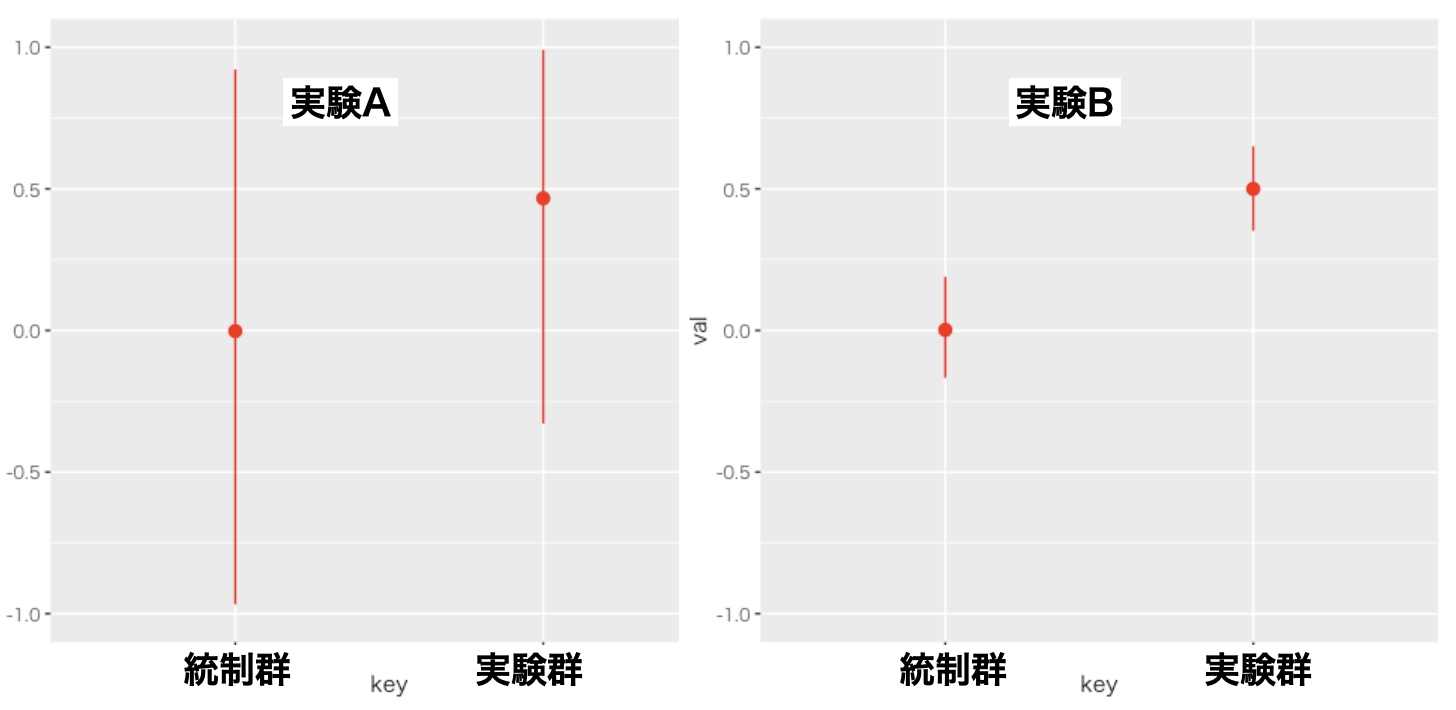
\includegraphics[keepaspectratio,width=0.8\linewidth]{../images/12_design1/slide12_05.png}
   \caption{Example of two experiments with the same difference in means (group effect). Which experiment is easier to say has an effect?}
   \label{fig::12_05}
\end{figure}


Please refer to Figure \ref{fig::12_05} here. It shows two sets of experimental results, Experiment A to the left and Experiment B to the right. This is a box-and-whisker plot where the red dots represent the means of each group and the lines extending above and below them connect the maximum and minimum values of each group.
You can easily see that Experiment A has a larger variance compared to Experiment B. Interestingly, the difference between the means of Experiment A and Experiment B is the same. In this case, which experiment can we definitively say had an effect?

Experiment A showed that on average, the experimental group had higher mean values than the control group. However, the maximum value in the control group is comparable to the numbers in the experimental group, and the minimum value in the experimental group could also be seen in the control group.
In contrast, Experiment B did not even reach the minimum value of the control group's maximum, no matter how hard they tried. It becomes easier to judge that the intervention by the experimental group was significant since they could not achieve a score as high as the experimental group's.

When evaluating whether there is an effect or not from an experiment, it is determined based on whether the variance between groups is sufficiently large compared to the variance within groups, without modifying the TeX code (see Figure 21-08).
\begin{figure}[ht]
   \centering
   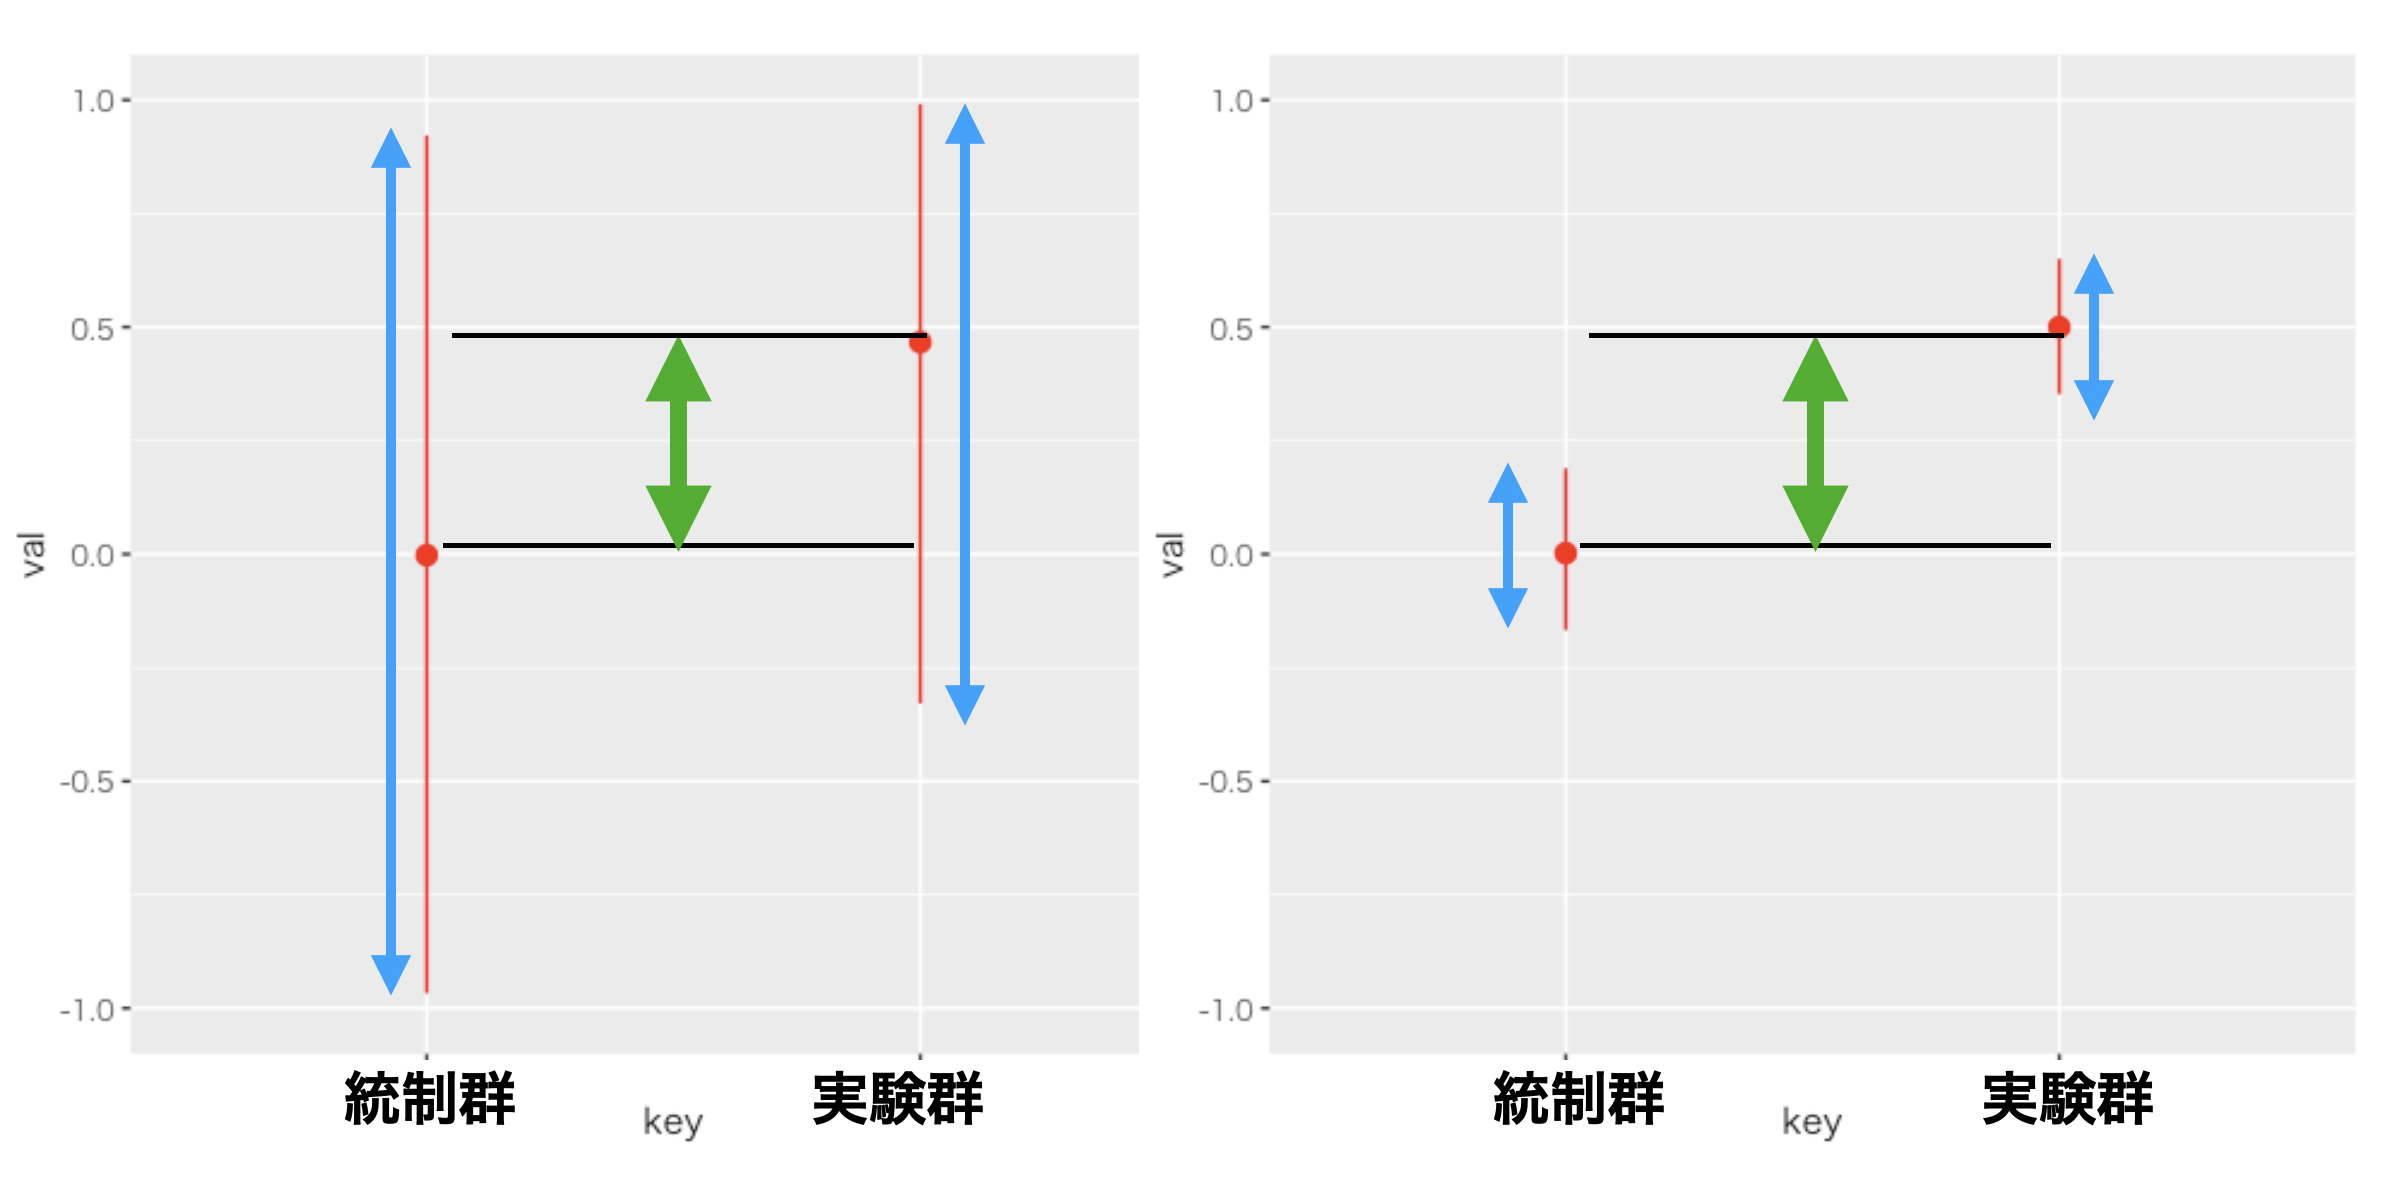
\includegraphics[keepaspectratio,width=0.8\linewidth]{../images/21_anova/slide21_08.png}
   \caption{Example of two experiments where the difference in mean (group effect) is the same. In the left example, it is difficult to say that there is an effect because the variation within groups (blue arrow) is greater than the variation between groups (green arrow). In the right example, it is easy to say that there is an effect since the maximum value in the control group is not even as high as the minimum value in the experimental group.}
   \label{fig::21_08}
\end{figure}


This concept is also related to the reliability of classical test theory. The definition of reliability is the ratio of the variance of the true score to the total variance, which is expressed as the following equation without altering the TeX code:

\[ Rel = \frac{Var(t)}{Var(X)}=\frac{Var(t)}{Var(t)+Var(e)} \]

The evaluation of the effect of an experiment is also expressed in terms of the relationship between the total variance $SS_t$, the between-group variance (or variance of effects) $SS_f$, and the error variance $SS_e$. This can be expressed as follows without modifying the TeX code.

\[ \frac{SS_f}{SS_t}=\frac{SS_f}{SS_f+SS_e} \]

The idea of decomposing variance and evaluating its ratio is also known as \keytermE{analysis of variance}, which has become a classical and fundamental research method in psychology.

\section{Task}
\paragraph{Factors and Levels} How would you design a psychology experiment using a factorial design? Please accurately express with attention to the difference between the words "factors" and "levels".

You are a translator.

\begin{itemize}
   \item アサガオの生長を観察するため、水をあげる群とあげない群、肥料をあげる群とあげない群をつくり、成長の程度を比較した。
   \item ラットの種類A/Bそれぞれに対して，トランキライザーの効果を見るため，0.4mg/0.7mg/1.5mg投与する群を作り比較した。
   \item 4つの学校で，1年間で共通の試験を実施した。一学期，二学期，三学期の各校における成績変化を比較したい。
   \item 二つの社会的強化の方法(a1,a2)があり，この条件に無作為に大学生を選び割り当てた。被験者は4つのセッション(b1,b2,b3,b4)を体験し，各セッションの作業量を調べ，比較する。
\end{itemize}

\paragraph{Calculating the Effect} The results of the common test conducted in the three schools in the previous example are shown in Table \ref{tbl:m12_example} (there were only four students in each school!). Let's calculate the difference (size of effect) between each school's overall average and group average, as well as the size of each individual's error. We will not modify the TeX code.
\begin{table}[ht]
   \centering
   \caption{一要因3水準Between計画のデータを分解する}
   \begin{tabular}{lccccc}
      \hline
      School & ID & Score & 群平均 & 効果 & 誤差 \\
      \hline
      A      & 1  & 58    &     &    &    \\
      A      & 2  & 58    &     &    &    \\
      A      & 3  & 64    &     &    &    \\
      A      & 4  & 56    &     &    &    \\
      B      & 1  & 53    &     &    &    \\
      B      & 2  & 53    &     &    &    \\
      B      & 3  & 54    &     &    &    \\
      B      & 4  & 53    &     &    &    \\
      C      & 1  & 39    &     &    &    \\
      C      & 2  & 38    &     &    &    \\
      C      & 3  & 35    &     &    &    \\
      C      & 4  & 38    &     &    &    \\
      \hline
   \end{tabular}
   \label{tbl:m12_example}
\end{table}



\end{document}
